\documentclass[preprint2,numberedappendix,tighten,twocolappendix]{aastex6}  % USE THIS TO MAKE BIB, THEN FORMAT USING EMULATEAPJ
%\documentclass[twocolumn,apj,numberedappendix]{emulateapj}
\shorttitle{Adding Sensitivity to 21cm Inteferometric Probes of Reionization}
\shortauthors{Zhang\&Parsons}
\usepackage{float}
\usepackage{amsmath}
\usepackage{graphicx}
\usepackage[figuresright]{rotating}
%\usepackage{rotating}
\usepackage{natbib}
%\usepackage{pdflscape}
%\usepackage{lscape}
\usepackage{ctable}
\citestyle{aa}
\renewcommand\[{\begin{equation}}
\renewcommand\]{\end{equation}}


\begin{document}

\title{Adding Sensitivity to 21cm Inteferometric Probes of Reionization by Optimizing Choice of Baselines}

%\maketitle
\author{
Yunfan Gerry Zhang \altaffilmark{1},
Aaron R. Parsons\altaffilmark{1}\altaffilmark{2}
}

\altaffiltext{1}{Astronomy Dept., U. California, Berkeley, CA}
\altaffiltext{2}{Radio Astronomy Lab., U. California, Berkeley, CA}

\begin{abstract}
We introduce an accurate method to extract additional sensitivity from data of redundant radio arrays. 
Using the latest and final 128-element version of Precision Array for Probing the Epoch of Reionization (PAPER-64), we illustrate 
how our method finds optimal baselines to cross correlate, including baselines that are slightly different in length and orientation. 
We predict the sensitivity improvements of including each baseline pairs. The extremely natural and simple implementation of this method
would increase the sensitivity of PAPER-128 by up to [~50] percent. 
\end{abstract}

\section{Introduction}

The epoch of reionization, or cosmic dawn represents the last key
stage of the universe's early evolution. Study of this event stands at
the intersection of cosmology and astrophysics. Understanding this
event is important not only as a scientific goal
of its own, but also because it potentially provides crucial information
to fundamental nature of inflation, neutrino mass and phenomenology
of the first stars and galaxies alike (e.g. \cite{LiuOpticalDepth}). 

Arguably the most promising observational probe of the epoch of reionization
comes from measurement of the ``spin-flip'' transition of neutral
hydrogen of characteristic wavelength 21cm \cite{Furlanetto2006181,PritchardLoeb}.
While probes such as quasar spectra rely on emission and scattering
of free electrons, and are thus limited to the lower redshifts after
the completion of reionization, the 21cm line directly probes the
abundance and distribution of neutral hydrogen, and thus would potentially
shed light on all stages of reionization. Radio interferometry efforts
to measure the 21cm power spectrum has been a top priority in recent years of astronomy.
Current generation instruments include the Precision Array for Probing
the Epoch of Reionization (PAPER) \cite{Ali2015,paper32}, Murchison
Widefield Array (MWA) \cite{MWA}, Low Frequency Array (LOFAR) \cite{LOFAR},
and next generation instruments such as the Hydrogen Epoch of Reionization
Array (HERA) (e.g. \cite{HERA,HERAconfiguration,HERABEAM1,HERADISH2})
and the Square Kilometer Array Low (SKA low) (e.g. \cite{SKA1}) are
under construction. 

One of the main challenges of interferometric observations of cosmic
21cm line is the foreground contamination. Both sources within our
galaxy, and to a lesser distant sources outside of our galaxy emit
radio contaminations (via for example synchrotron processes) up to five orders of magnitude stronger than the
reionization signal. There are two common methods to deal with the
foreground contamination. In the first, sometimes called the foreground
removal technique, individual sources are identified and removed in the image domain.
The other technique, commonly referred to as 'foreground avoidance',
makes use of the fact that most common foreground contaminations have a smooth
spectrum, and thus is constrained to a Fourier domain ``foreground
wedge'' \cite{wedge1,wedge2}. Thus contamination can be avoided
by restricting our observation to ``outside the wedge'', where the data is currently noise dominated. The main
challenge of using the avoidance technique is thus the sensitivity, or
the signal to noise ratio. This is the motivation for the design of
the maximum redundancy arrays such as PAPER and HERA. While traditional
imaging arrays focus on Fourier mode uv coverage, the redundant arrays
focus on redundant measurements of the same Fourier mode
with many tightly packed antennas at equal spacing. Since baselines
of the same length and orientation measure the same Fourier modes
on the sky, the maximum redundancy arrays is able to increase the
signal to noise ratio by averaging over measurements of the same baseline.
\cite{Ali2015} provides the newest upper limit to the power spectrum
measurements with the PAPER-64 data. From some models we roughly expect
that the sensitivity required for detection is a factor of 10 away.
This paper explores a new technique to add sensitivity to the analysis
of redundant arrays, by making use of the earth's rotation. This technique
can be applied to redundant arrays such as PAPER and HERA to increase
the sensitivity by up to a factor of [1.5]. 

The earth's rotation causes the baselines to pick up different modes of the sky with time. 
This effect is used extensively to improve uv coverage in imaging with minimum redundancy arrays. In
a maximally redundant array, baselines that are slightly different
rotate into each other at a time delay. Here we present a method to
improve the sensitivity of the maximum redundancy arrays by considering
the uv redundancy of different baselines at a time lag. 

Baselines of the same length and orientation are traditionally called
``redundant baselines'', because they measure the same Fourier mode
in the sky. In order to eliminate confusion and ambiguity, we shall
introduce slightly different terminology. We'll call baselines that
are the same length and orientation ``equivalent baselines'', inspired
by the mathematical notion of equivalency classes. Two equivalent
baselines will be redundant with each other simultaneously at all
times. Some non-equivalent baselines can also be redundant if their
respected time series is shifted with respect to one another by a
certain delay. In other words, one baseline can be ``rotated into''
another. We call these ``near-equivalent baselines''. It is our
goal to a) identify the near-equivalent baselines that give good
redundancy, b) to find the optimal time offset for a given pair of baselines, and
c) to quantify the sensitivity improvement associated with cross multiplying
such a pair of near-equivalent baselines. In section
2 we explain the theoretical basis for this cross multiplication.
In section 3 we present details of the numerical implementation of
this technique. In section 4 we discuss the expected sensitivity improvement
with this method and with section 5 we conclude. 


\section{Method}

\subsection{Rough Idea}
\begin{figure}[H]
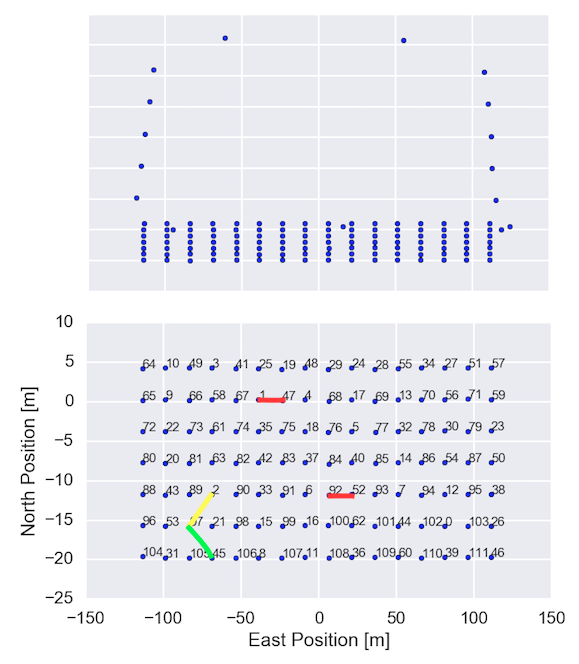
\includegraphics[width=\linewidth]{antpos128}

\caption{The PAPER-128 layout. Each blue dot corresponds to the location of
an antenna. Top panel shows the antenna positions drawn to scale,
bottom panel show the antenna labels and distances, excluding the outlier
antennas.\label{fig:AntPos}
The numbering of the antennas the bottom panel are original labels
during instrument assembly and does not bear significant
meaning. Baselines corresponding to the same separations are called
equivalent. In the bottom panel, the two baselines labeled with the
red arrow are equivalent, with separation denoted by sep1,0, for the
antennas are separated by 1 unit east and 0 unit north. Similarly,
the baselines labeled with the yellow and green arrows are examples
of sep1,1 and sep-1,1, respectively. Note sep1,0 and sep-1,0 for example
are the same baselines and should not be counted twice.}
\end{figure}


We shall use the 128-element PAPER array to demonstrate. 
The PAPER array is located in the Karoo desert in South Africa (30:43:17.5
S, 21:25:41.8 E). The layout pattern with antenna labels are show
in Fig. \ref{fig:AntPos}. We see the antenna spacing in North-South
directions are comparatively close (4m), so that baselines such as
0\_44 and 0\_7 are very close to equivalent. In the bottom panel,
the two baselines labeled with the red arrow are equivalent, with
separation denoted by sep1,0, for the antennas are separated by 1
unit east and 0 unit north. Similarly, the baselines labeled with
the yellow and green arrows are examples of sep1,1 and sep-1,1, respectively.
Note sep1,0 and sep-1,0 for example are the same baselines and should
not be counted twice. Turns out antennas in purely north-south baselines
are close enough to induce cross talks, and hence are not suitable
for use. The original PAPER-64 analysis used three classes of baselines, here
equivalent to 
sep2,0, sep2,1 and sep-2,1 \cite{Ali2015}. There each of these classes
of baselines are cross multiplied to itself. We shall see that in addition these
baseline classes can be cross multiplied with a time offset.


Given a point source on the sky, each baseline maps the
source to a point in uv plane. As the earth rotates with respect to
the source, the point traces out tracks in the uv-plane. 
The uv tracks of PAPER-128 over 7.2 hours, at 0.15GHz, for a source that passes through zenith, are shown in Fig. \ref{fig:Tracks}. 


\begin{figure}[H]
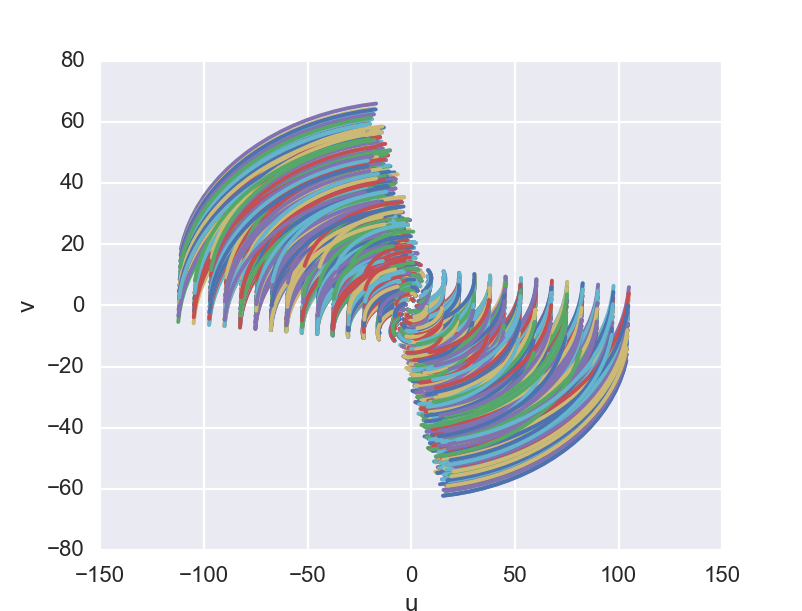
\includegraphics[width=\linewidth]{tracks128}
\caption{Tracks of PAPER-128 (grid only, excluding outliers) for a hypothetical source that passes through zenith.
These tracks are traced out over 0.2 sidereal days, or roughly 4.8
hours. Color represents different baselines. Frequency is $\nu=0.15\text{GHz}$.
As the earth rotates, tracks are traced out counterclockwise. \label{fig:Tracks}}
\end{figure}

Roughly speaking, we can identify
redundancy of near-equivalent baselines as crossings
of the uv tracks. Although this is a valid quick method to identify some baselines to cross-multiply, we find
that it is not accurate enough for time offset determination. The reason is, for wide beam antennas such as PAPER, the sources are not point-like. 
In other words, when tracks of
one point of the sky are crossing in uv-plane, those corresponding to another is not. To accurately
constrain redundancy we must take into account of finite beam width. A more rigorous treatment is thus required.  
We show the beam of PAPER antennas in Fig.\ref{fig:Beam} for reference:

\begin{figure}[H]
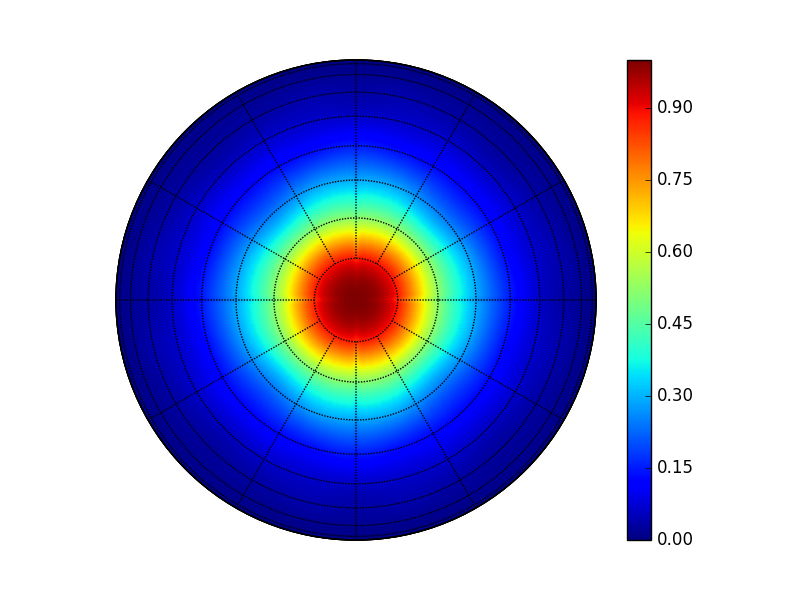
\includegraphics[width=\linewidth]{BEAM}

\caption{Beam of PAPER antennas. Shown here is the values of $A$ (Eq. \eqref{eq:Vis1})
for frequency of $\nu=150\text{MHz}$. Notice $A$ is a ``baseline's
beam''. Since all antennas in PAPER have the same beam, $A$ here
is just the square of an antenna beam, and is normalized to 1 at the
center. The circles centered around zenith (center of beam) here are
spaced 10 degrees apart. Such a wide beam limits the accuracy of the uv track-crossing as a method of redundancy search. \label{fig:Beam}}
\end{figure}



\subsection{Formalism}
Below we shall derive theoretical expectations of cross multiplications
of two near-equivalent baselines. More precisely we shall relate
the product of visibilities of two different baselines to the power spectrum. 


We take the visibility as commonly defined in the literature (e.g.
\cite{first-paper}): 
\begin{equation}
\begin{aligned}V_{\nu}(b) & =\int d\Omega A_{\nu}(\hat{s})\phi(\nu)I_{\nu}(\hat{s})\exp\left[-2\pi i\frac{\nu}{c}b\cdot\hat{s}\right],\\
 & \approx\frac{2k_{B}}{\lambda^{2}}\int d\Omega A_{\nu}(\hat{s})\phi(\nu)T(\hat{s})\exp\left[-2\pi i\frac{\nu}{c}b\cdot\hat{s}\right],
\end{aligned}
\label{eq:Vis1}
\end{equation}
Here $\lambda$ is a mean wavelength, $\boldsymbol{b}$ is the baseline
length, $\hat{\boldsymbol{s}}$ and $\Omega$ are a direction in the
sky and its corresponding solid angle. $A_{\nu}$ is the (frequency
dependent) beam, and $I$ is the specific intensity, which has been
related to $T$, the brightness temperature in the Rayleigh-Jeans
limit. $\phi(\nu)$ is the frequency band profile. For PAPER-64, for example,
the bands studied are roughly a top-hat from 144MHz to 154 MHz. 

We define the delay transformed visibility \cite{delay-transform}:
\small
\begin{equation}
\begin{aligned}V(b,\tau) & =\int d\nu V_{\nu}(b)\phi(\nu)\exp\left[-2\pi i\nu\tau\right],\\
 & =\frac{2k_{B}}{\lambda^{2}}\int d\Omega d\nu A(\hat{s},\nu)\phi(\nu)T(\hat{s},\nu)\exp\left[-2\pi i\nu\left(\frac{b\cdot\hat{s}}{c}+\tau\right)\right]
\end{aligned}
.\label{eq:Vb1}
\end{equation}
\normalsize


Eq. \eqref{eq:Vb1} expresses the delay-transformed visibility as
an integral over observation coordinates $\hat{s}$ and $\nu$. Ultimately,
we would like to relate the data, collected with coordinates $\hat{s}$
and $\nu$, to the power spectrum, written with cosmological coordinates
$\boldsymbol{r}$ and $\boldsymbol{k}$. We start by noticing that
{[}Gerry: change all r and k into bold{]} 
\[
\begin{aligned}r & =\frac{c}{H_{0}}\int_{0}^{z}\frac{dz'}{E(z')},\\
 & \approx\frac{c}{H_{0}}\int_{0}^{z_{0}}\frac{dz'}{E(z')}-\frac{c(1+z)^{2}}{\nu_{21}H_{0}E(z)}\left(\nu-\nu_{0}\right),\\
 & \equiv D_{c}-Y\Delta\nu,
\end{aligned}
\]
where $\nu_{21}=1420MHz$ is the 21cm transition rest frequency, $\nu_{0}$
a reference central frequency with corresponding redshift $z_{0}$,
and 
\[
E(z)=\sqrt{\Omega_{m}(1+z)^{3}+\Omega_{\Lambda}}.
\]
Inverting for $\nu$:
\begin{equation}
\nu=\frac{D_{c}-r}{Y}+\nu_{21}.\label{eq:nur}
\end{equation}
Thus $d\nu=-dr/Y$ and $d^{3}r=-X^{2}Yd\Omega d\nu$. 

We can thus rewrite the delayed transformed visibility as 
\small
\[
\boxed{\begin{aligned}V(b,\tau) & =\frac{1}{X^{2}Y}\int_{H}d^{3}rA(\vec{r})\phi(r)I(\vec{r})\exp\left[-2\pi i\left(\frac{b}{c}\cdot\hat{r}+\tau\right)\nu_{r}\right]\end{aligned}
}.
\]
\normalsize
Here $(r_{x},r_{y},r_{z})=(X\hat{s}_{x},X\hat{s}_{y},Y\nu)$, and
$(Xk_{x},Xk_{y},Yk_{z})=\frac{2\pi}{c}(b_{x},b_{y},\eta)$ relate
the cosmological coordinates $r$ and $k$ to the measured coordinates.
We have written $\nu_{r}$ to remind us that $\nu$ and $r$ are related
by Eq. \eqref{eq:nur}. The beam reception pattern $A$ is dimensionless,
normalized to 1 at its peak (zenith), and we assume it to be the same
for all baselines. 

With a time offset, the beam pattern has moved relative to the sky.
Here we choose to fix the sky, and denote the rotated coordinates
of the beam pattern with the operator $\Gamma$. With implicit bounds
of integrals from $-\infty$ to $\infty$, we have:
\begin{widetext}
\begin{equation}
\begin{aligned} & \langle V^{*}(b,\tau)V(b',\tau')\rangle\\
 & =\left(\frac{2k_{B}}{X^{2}Y\lambda^{2}}\right)^{2}\int d^{3}rd^{3}r'\left(\langle T^{*}(r)T(r')\rangle\right)A^{*}(r)A(\Gamma r')\Phi_{b,\tau}(r,\Gamma r'),\\
 & =\left(\frac{2k_{B}}{X^{2}Y\lambda^{2}}\right)^{2}\int d^{3}rd^{3}r'\left(\int\frac{d^{3}\kappa}{(2\pi)^{3}}\frac{d^{3}\kappa'}{(2\pi)^{3}}\langle T^{*}(\kappa)T(\kappa')\rangle e^{-i(\kappa r-\kappa'r')}\right)A^{*}(r)A(\Gamma r')\Phi_{b,\tau}(r,\Gamma r'),\\
 & =\left(\frac{2k_{B}}{X^{2}Y\lambda^{2}}\right)^{2}\int d^{3}rd^{3}r'\left(\int\frac{d^{3}\kappa}{(2\pi)^{3}}P(\kappa)e^{-i\kappa(r-r')}\right)A^{*}(r)A(\Gamma r')\Phi_{b,\tau}(r,\Gamma r'),\\
 & =\left(\frac{2k_{B}}{X^{2}Y\lambda^{2}}\right)^{2}\int d^{3}rd^{3}r'\xi(r-r')A^{*}(r)A(\Gamma r')\Phi_{b,\tau}(r,\Gamma r'),\\
 & \approx\left(\frac{2k_{B}}{X^{2}Y\lambda^{2}}\right)^{2}P(k_{b,\tau})\int d^{3}rd^{3}r'\delta_{D}^{(3)}(r-r')A^{*}(r)A(\Gamma r')\Phi_{b,\tau}(r,\Gamma r'),\\
 & =\left(\frac{2k_{B}}{X^{2}Y\lambda^{2}}\right)^{2}P(k_{b,\tau})\int d^{3}r|A^{*}(r)A(\Gamma r)||\phi(\nu_{r})|^{2}\exp\left[-i2\pi\nu_{r}\left(\hat{r}\cdot\frac{b}{c}-\hat{\Gamma r}\cdot\frac{b'}{c}\right)\right],\\
 & =\left(\frac{2k_{B}}{\lambda^{2}}\right)^{2}P(k_{b,\tau})\int\frac{d\Omega d\nu}{X^{2}Y}|A^{*}(\hat{s},\nu)A(\hat{\Gamma s},\nu)||\phi(\nu)|^{2}\exp\left[-i2\pi\nu\left(\hat{s}\cdot\frac{b}{c}-\hat{\Gamma s}\cdot\frac{b'}{c}\right)\right],
\end{aligned}
\label{eq:main}
\end{equation}

where in transition from cosmological coordinates back to observing coordinates we have written $\hat{r}\equiv\hat{s}$, and 
\begin{equation}
\Phi_{b,\tau}(r,\Gamma r')=|{\phi^{*}}(\ensuremath{\nu_{r}})\phi(\nu_{r'})|\exp\left[-i\frac{2\pi}{c}\left(b\cdot\nu_{r}\hat{r}-b'\cdot\nu_{r'}\Gamma\hat{r'}\right)\right]\exp\left[-i2\pi\tau\left(\nu_{r}-\nu_{r'}\right)\right].
\end{equation}
\end{widetext}
The second to third line of Eq.(\ref{eq:main}) follows from assumption of Gaussian random
sky, and the third to fourth line follows from the assumption that
the 3D power spectrum varies negligibly over the region of interest
so that $\hat{P_{21}}(k+k_{2})\approx\hat{P_{21}}(k)$. Since $\Gamma$
is a sky rotation, it doesn't affect $\nu$, hence we have taken $\nu_{r}$
outside the parenthesis. Notice that the phase factor $\exp\left[-i2\pi\eta\left(\nu-\nu'\right)\right]$
drops out in the end. 

Finally, since the beam pattern and bandwidth are given in $\hat{s}$
and $\nu$, we convert the integral back to these coordinates to get
the general relation between the delay-transformed visibilities and
the power spectrum:

\begin{equation}
\boxed{\begin{aligned} & \langle V^{*}(b,\tau)V(b',\tau')\rangle\\
 & =\left(\frac{2k_{B}}{\lambda^{2}}\right)^{2}P(k_{b,\tau})\int\frac{d\Omega d\nu}{X^{2}Y}|A^{*}(\hat{s},\nu)A(\hat{\Gamma s},\nu)||\phi(\nu)|^{2}\\
 & \qquad \qquad \qquad \qquad \exp\left[-i2\pi\nu\left(\hat{s}\cdot\frac{b}{c}-\hat{\Gamma s}\cdot\frac{b'}{c}\right)\right].\end{aligned}}
\label{eq:final}
\end{equation}
So roughly speaking the cross multiplications of visibilities at a time delay
in uv-space is proportional to the power spectrum times the Fourier
transform of the cross multiplied beam pattern. We can then in principle
combine information from different baseline pairs if we correct for
the phase and normalization. As a check, when applied to equivalent baselines,
$b=b'$, $\hat{s}=\hat{\Gamma s}$, and Eq.(\ref{eq:final}) reduces to Eq.(B9) of \cite{paper32}. 

If this result is robust, then we can achieve all our goals stated in the introduction, i.e. to identify 
candidate baseline pairs, to find the optimal time offset, and to quantify the sensibility, by computing the integral
in Eq.(\ref{eq:final}) for various time offsets. Thus we shall first test its robustness numerically.


\section{Analysis}
\subsection{Numerical Test \label{sec:Techniquet}}

To test the robustness of Eq.(\ref{eq:final}), we need to compare the amplitude and phase of the integral
for a pair of baselines with products of simulated visibilities of those baselines. 

For the simulation, we take N random realizations of the sky
on a healpix map (\cite{Heal}, \cite{HealPrimer}) \footnote{We use functionalities in the python package AIPY for healpix mapping
as well as coordinate transforms. }. For each realization, each pixel is given a Gaussian random value
of brightness temperature. We then rotate the baseline positions with
the appropriate rotation matrix, recording the visibilities, for each
baseline \footnote{As a caveat, there are two obvious ways to achieve the rotation. One
can either fix the sky and rotate the baselines, or the other way
around. We found however, that we must not physically rotate the sky
map, for the numerical round-offs due to finite resolutions of the
map turns out to be significant. Thus we let the sky, represented
by the healpix map, be fixed, and rotate the baselines. }. The resulting visibilities for the two baselines are then convolved
via the Fourier convolution theorem, to obtain values of the cross
correlation as a function of time-offset. The peak of the curve then
corresponds to maximum redundancy. The accuracy of this result is
limited by (simulated) cosmic variance and finite spacial resolution,
and hence can be beat down by averaging over a large number of universes.
A numerical estimate of the error of the peak height with $N=1$ is
$\lesssim20\%$, and thus with $N=2500,$ we achieve an error of peak
height $<0.5\%$. 

To test our understanding of the time-offset, and to verify our derivation
in Eq. \eqref{eq:main}, we must compare the simulated visibility cross multiplication with the integral in
Eq. \eqref{eq:main}, for a pair of near-equivalent baselines. 
This comparison is show in Fig. \ref{fig:numerics}. 
Since the sensitivity contribution is inferred from height of the peak of the cross-multiplied visibilities as a function of time. 
We first compare the simulation to the integral for a pair of equivalent baselines, then normalize the peaks 
of the near-equivalent baselines to that of the equivalent ones. 
In Fig. \ref{fig:numerics}  we show on the top comparison of
the convolution of an equivalent baseline, normalized to 1 at the
peak, whose location is at zero time offset as expected. On the bottom we show
comparison of a near-equivalent baseline pair, of classes sep1,0:1,1 and sep1,1:1,1. The peaks
are normalized with the same factor as the peak height on the top,
i.e. the two plots have thus the same scale on the vertical axis.
The height of the plot on the right thus quantifies the added sensitivity. 

\begin{figure}[H]
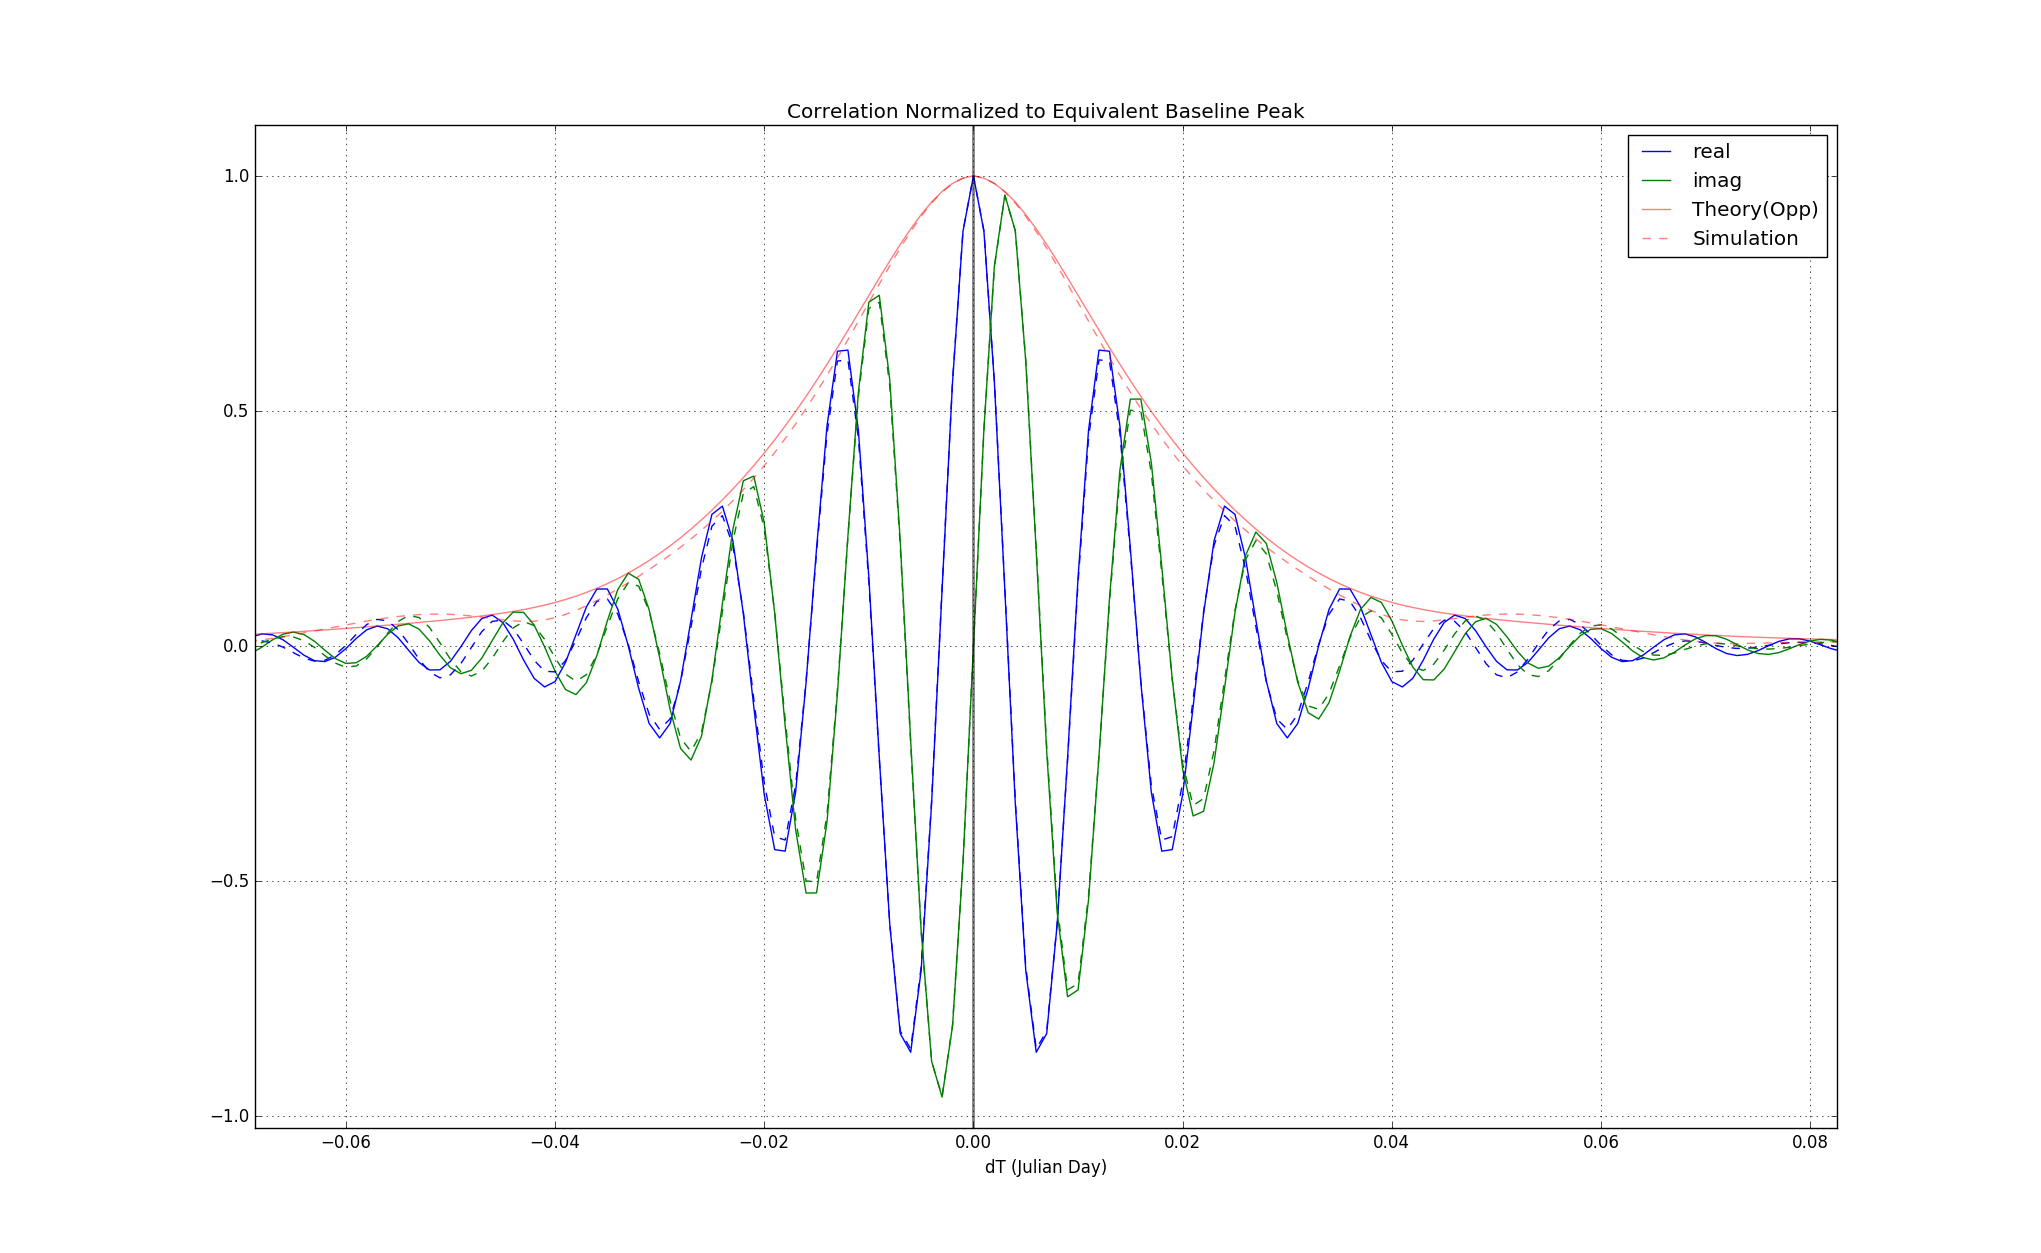
\includegraphics[width=\linewidth]{redun_agree}
\label{fig:numerics}
\caption{[Placeholder Plot]}
\end{figure}


At the optimal time separation, the integral in Eq. \eqref{eq:final}
is maximized. Thus as a final check we expect the two beams to have to same fringe pattern
(frequency and phase). Due to the time delay, however, the beam center
would be slightly shifted with respect to each other. This we show
in Fig. \ref{fig:Beam-fringe-pattern}. The left and middle panels show the beam fringe
patterns for baselines sep0,1 and sep1,1, delayed by 0.0325 days,
and the right panel shows their cross product. The fringe pattern
indeed cancels out as we expect. 

\begin{widetext}
\begin{figure}[H]
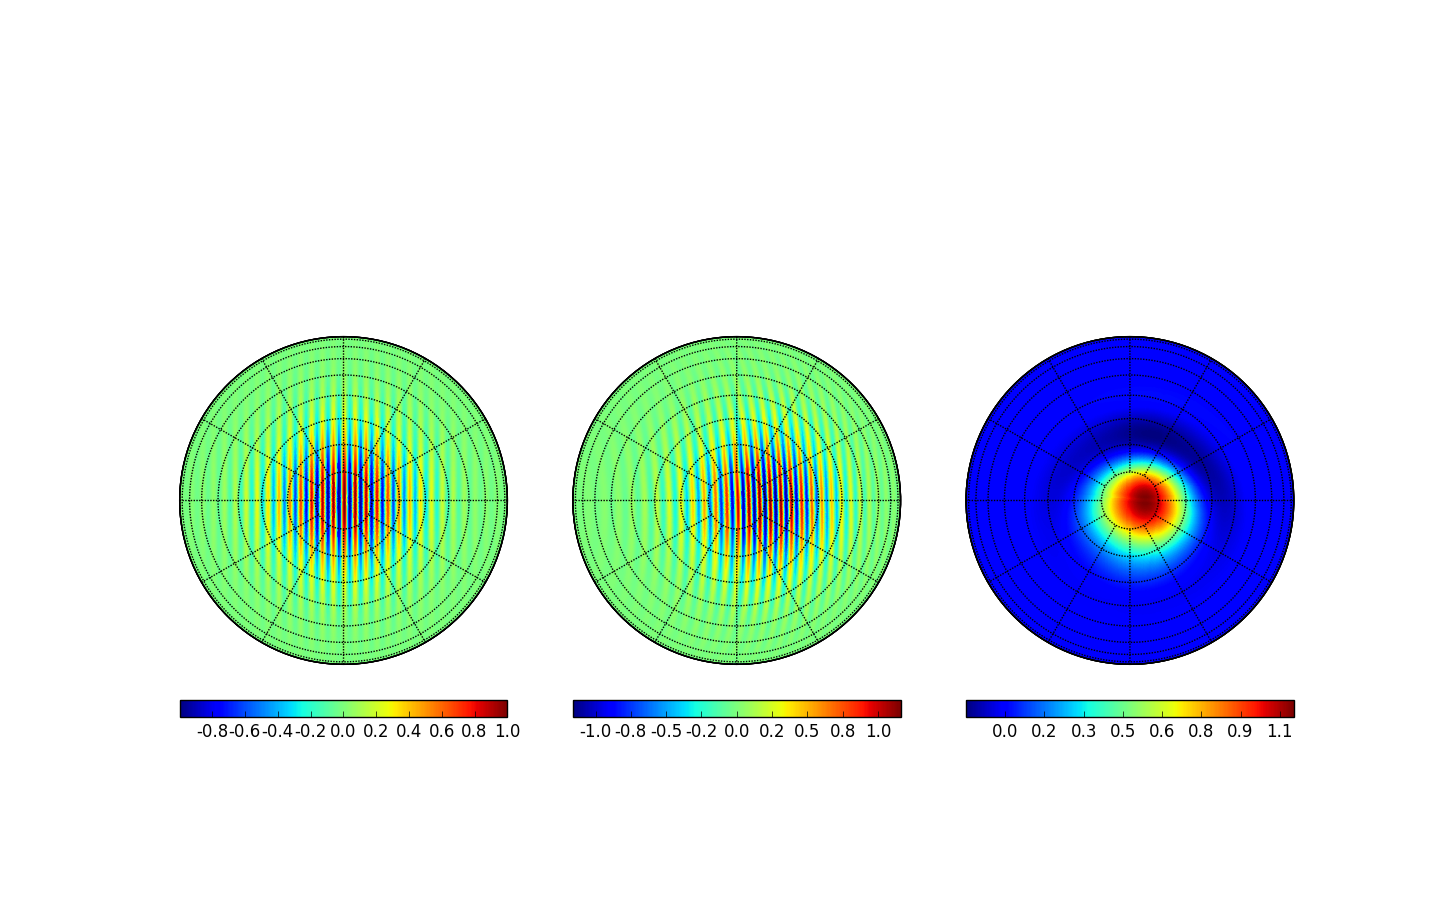
\includegraphics[scale=0.5]{fringe_res}

\caption{Beam fringe pattern of sep1.0(left), sep1,1 at a time delay (middle),
and their conjugate product. Frequency of $\nu=0.15\text{GHz}$ is
chosen. \label{fig:Beam-fringe-pattern}}
\end{figure}
\end{widetext}




\subsection{Expected Sensitivity Contributions}

Having verified Eq. \eqref{eq:main}, we can thus predict the sensitivity contributions of a
particular baseline pair simply by computing the integral. 
Having computed all of the baseline pairs, we find that baseline pairs that are mirror images of each other 
give the same amount of redundancies (peak height), with the opposite time offset, as expected from symmetry. 
For example, sep1,0:1,1 is mirror image of sep1,0:1,-1 and thus these two baseline pairs
give the same sensibility contribution. Thus in our results we shall only show a subset of representative baseline pairs 
that give different informations. 

In the top panel of Fig. \eqref{fig:sensplot} below
we show the peak heights and locations for a variety of baseline combinations.
We see that baseline pairs that have crossings at a smaller time delay
tend to have higher correlations. In other words, correlation peaks
that are closer to zero time lag are higher. This is expected since
a) the longer the time delay, the more the antennas have moved with respect
to the sky and hence the less overlaps in patch of sky surveyed, b) smaller optimal
time-offset corresponds to smaller differences in orientation, and hence in length of
baselines in PAPER-64. 

\begin{figure}[H]
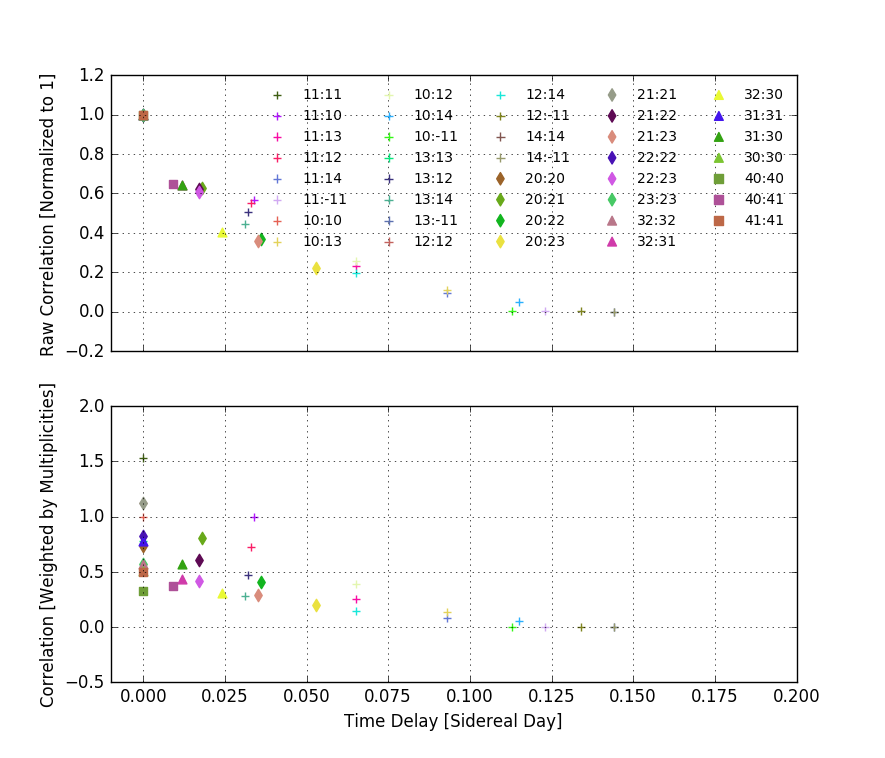
\includegraphics[width=\linewidth]{sensitivity}
\label{fig:sensplot}
\caption{Relative sensitivity contributions of selected baseline combinations in PAPER-64. In the legend m,n:p,q denotes cross
multiplying PAPER-64 baselines of east-west, north-south separations (m,n) and (p,q) respectively. The top
panel shows the peak height (degree of correlation) of each baseline
combination, while the bottom panel multiplies the heights by the
corresponding multiplicities as in Eq. \eqref{eq:sensul}, and in some cases an extra factor of 2 (explained in text). 
In weighting by the multiplicity (bottom), we have chosen to fix the sensitivity 
contribution of 1,0:1,0 to unity. }


\end{figure}


To determine that actual relative contribution to sensitivity of these
baseline pairs, we have to take into account of the multiplicities of
these baselines, or the size of the equivalency classes in a mathematical
language. By these we mean how many physical antenna pairs have the
same length and orientation. Looking at Fig. \ref{fig:The-PAPER-64}
we see for example sep1,0 will have higher redundancy than sep2,0,
or sep1,1. The latest release of PAPER-64 data uses baselines sep-1,1,
sep0,1 and sep1,1 \cite{Ali2015}, and achieved a $2\sigma$ upper
limit of $22.4mK^{2}$. There, the three sets of equivalent baselines
are only cross multiplied by itself. Assuming that each baseline delivers
the same quality of data (i.e. they have the same height of correlation
peaks, which is in our normalization equal to unity), the relative
contribution to sensitivity can be estimated. 

First we can average of the visibilities of the baselines of the same
separations. Since PAPER-64 has 8 by 8 antenna configuration, there
are $(8-|m|)\times(8-|n|)$ copies of the baseline sepm,n. This means
that if we add visibility measurements of all these equivalent baselines,
we get a factor of $\sqrt{(8-|m|)\times(8-|n|)}$ reduction in noise
level. The sensitivity contribution of sepm,n, being the signal to
noise ratio of the power spectrum, is thus proportional to $(8-|m|)\times(8-|n|)$.
Next we can average over the power-spectrum taken from baselines of
the different separations. Thus the total cumulative sensitivity is
given by 
\begin{equation}
\frac{P_{S}}{P_{N}}\propto\sqrt{\sum_{(n,m)}\left((8-|m|)\times(8-|n|)\right)^{2}},\label{eq:sensequiv}
\end{equation}
where the sum is only over pairs of m and n. If we now include power
spectrum from cross-multiplications of near-equivalent baselines of
types sepm,n and sepm',n', we get a general cumulative sensitivity:
\small
\begin{equation}
\frac{P_{S}}{P_{N}}\propto\sqrt{\sum_{(n,m,n',m')}\Omega_{mnm'n'}\left((8-|m|)(8-|n|)(8-|m'|)(8-|n'|)\right)},\label{eq:sensul}
\end{equation}
\normalsize
where $\Omega$ is the correlation peak height show in top panel of Fig. \eqref{fig:sensplot},
and the sum is again only over tuples of m,n,m',n'. This form now
includes the equivalent baselines in Eq. \eqref{eq:sensequiv}, with
$\Omega_{m=m',n=n'}=1$. 
Shown in the bottom panel of Fig. \eqref{fig:sensplot} is the peak heights weighted
by this multiplicity factor (before taking the square root), with one difference. The difference is, 
since we have "folded over" the negative time delays, we have combined baseline pairs that are identical modulus parity, 
or in other words are mirror images of each other, by summing over them to get an extra factor of two. For example, 
instead of plotting 1,1:1,1 and 1,-1:1,-1 separately, we plot 1,1:1,1 with twice the multiplicity. Similarly, baseline pairs such as 
1,0:1,1 also get the factor of 2 because they are identical to 1,0:1,-1. Baseline pairs such as 1,0:1,0, or 1,1:1,-1 do not get
the factor of 2 because their mirror images are themselves. 

\subsection{Validation with PAPER-128 Data}

\section{Conclusion}

\bibliographystyle{apj}
%\nocite{*}
\bibliography{draft_working}

\end{document}
